% TMLR submission, anonymous form. Use \usepackage[preprint]{tmlr} or [accepted] to reveal authors.
\documentclass[10pt]{article}
\usepackage{tmlr}
\usepackage{microtype,graphicx,booktabs,url,amsmath,amssymb,amsfonts,amsthm}
\usepackage{algorithm}
\let\AND\relax
\usepackage{algorithmic}
\usepackage{longtable}
\usepackage[hidelinks]{hyperref}
\newtheorem{proposition}{Proposition}
\newcommand{\NStreams}{20}
\newcommand{\NEpisodes}{307}
\newcommand{\NCheaper}{19}
\newcommand{\NEqual}{0}
\newcommand{\NDearer}{1}
\newcommand{\MaxDearer}{0.22}
\newcommand{\MeanSaving}{37}
\newcommand{\MedSaving}{30}
\newcommand{\MaxSaving}{75}
\newcommand{\NPromoted}{18}
\newcommand{\MedSavingPromoted}{31}
\newcommand{\NOther}{2}
\newcommand{\MedSavingOther}{13}
\newcommand{\NSameEpisodes}{275}
\newcommand{\NSameStreams}{10}
\newcommand{\MedCostChange}{0.95}
\newcommand{\MeanCostChange}{1.43}
\newcommand{\NSixCheaper}{5}
\newcommand{\NBeatNever}{19}
\newcommand{\NIncBeatNever}{19}
\newcommand{\NLowPower}{2}


\title{What Does It Cost to Keep a Certificate? Label-Efficient Sequential Certification for Model
Switching under Budgeted and Delayed Feedback}

\author{\name Anonymous Authors \email anonymous@example.com \\
      \addr Anonymous Institution}

\def\month{MM}
\def\year{YYYY}
\def\openreview{\url{https://openreview.net/forum?id=XXXX}}

\begin{document}
\maketitle

\begin{abstract}
Sequential certificates let a challenger replace a deployed model as soon as paired-loss
evidence suffices, but under a label budget a certificate kept alive for rollback keeps buying
labels after the decision has settled: on a \texttt{spam} stream, a budgeted certified switching
procedure promotes the challenger at event~244 of 2000 on average and then spends its full
200-label budget. We propose \emph{settled-decision acquisition}, which attenuates the paced query
rate when the promoted challenger remains ahead and, as an optional pre-promotion safeguard, when
an optimistic bound on the challenger's advantage indicates that promotion would not recover its
switching cost. The construction of the evidence process, the promotion threshold and the rollback
test are unchanged,
so the type-I error bound of each certificate is preserved, and a positive query floor keeps
rollback monitoring at a minimum rate. On \NStreams{} real datasets (\NEpisodes{} episodes),
compared with the same procedure without the gate, it uses \MeanSaving\% fewer labels (median
\MedSaving\%), and deployment loss, switches and rollbacks are identical for the two procedures on
every query seed in \NSameEpisodes{} of \NEpisodes{} episodes. Net cost is lower on \NCheaper{} of
the \NStreams{} datasets (mean \MeanCostChange\%, median \MedCostChange\%); label spend is at most
10 of the 104 to 483 cost units per episode. The episode-bootstrap interval for the cost
difference lies below zero on 17 of the 18 datasets with at least five episodes.
\end{abstract}

\section{Introduction}
Under a label budget, a sequential certificate for replacing a deployed model keeps buying labels
after it has already changed the deployed action. Replacing a model requires purchased labels that
arrive late, each deployment switch incurs a cost, and the certificate allows promotion as soon as
enough paired-loss evidence has arrived. In the \texttt{spam} example in
Figure~\ref{fig:method}, a budgeted certified switching procedure with rollback promotes the
challenger at event~244 on average over query seeds and then spends its full 200-label budget
over the rest of the 2000-event episode. Once the challenger is deployed and remains ahead, those
labels mainly provide rollback monitoring.

Existing certified-update procedures either stop querying once the verdict is reached, and so
cannot roll back~\citep{karampatziakis2021offpolicy,balachandran2026discern}, or monitor a
deployed model without a label budget~\citep{podkopaev2022tracking}. We therefore construct
\textsf{P3b} (Section~\ref{sec:method}), which keeps its certificate alive for rollback under a
hard budget; on \texttt{spam} it spends most of its labels after the decision. Lowering its budget
would not remove that spend selectively, because a smaller budget also slows the pre-promotion
evidence that drives promotion. Cutting post-promotion spend is constrained in three ways: stopping
altogether removes rollback, labels arrive $d$ events late, and a query rule that reacts to the
evidence must not invalidate the test that the evidence feeds.

We address that acquisition decision with \emph{settled-decision acquisition}, which multiplies
the paced query probability by an acquisition multiplier $r_t$. The multiplier is zero in a
post-promotion \textsc{settled} state, when the recent paired advantage still favours the deployed
challenger, and $0.25$ in an optional pre-promotion \textsc{hopeless} state, when even an upper
confidence bound on the challenger's advantage cannot repay the switching cost. A positive query
floor retains monitoring, which answers the first constraint. The multiplier is computed only from
labels released before each event, so it stays predictable under any fixed delay $d$, and because
it enters only through that predictable propensity, the type-I error bound of each certificate is
preserved (Proposition~\ref{prop:validity}). The construction of the evidence process, its
propensity-matched bet cap
and the promotion and rollback tests are unchanged, so decisions differ only where the purchased
evidence differs.

Across \NStreams{} real datasets the gate uses \MeanSaving\% fewer labels than \textsf{P3b}
(median \MedSaving\%, up to \MaxSaving\%), and deployment loss, switch count and rollback count are
identical for the two procedures on every query seed in \NSameEpisodes{} of \NEpisodes{} episodes.
Measured against label spend the saving is large: on \texttt{metro} the ungated procedure spends
its full 10 cost units of labels and the gate saves 6.78 of them. Net cost is lower on \NCheaper{}
of the datasets, by \MeanCostChange\% on average (median \MedCostChange\%). Label spend is at
most 10 of the 104 to 483 cost units per episode.

\paragraph{Contributions.}
\begin{itemize}
  \item We propose settled-decision acquisition (Section~\ref{sec:method}), a state-dependent
  multiplier on the paced query rate of a budgeted certified switching procedure with rollback,
  and show that the type-I error bound of each certificate holds for any predictable multiplier
  (Proposition~\ref{prop:validity}).
  \item We evaluate the gate as an ablation of that procedure on \NStreams{} real datasets
  (Section~\ref{sec:results}), decompose every cost difference into loss, query and switch
  components, and show that on \texttt{spam} and \texttt{rialto} the saving is entirely due to
  the \textsc{settled} state (Section~\ref{sec:ablation}).
\end{itemize}

\section{Related Work}\label{sec:related}
\paragraph{Anytime-valid testing.} Our certificates are e-processes built by testing by
betting~\citep{shafer2021testing,vovk2021evalues,ramdas2023gametheoretic}, and the
$\log(1/\alpha)$ threshold is justified by Ville's inequality~\citep{ville1939etude}. Paired-loss
e-processes for comparing sequential forecasters are developed by~\citet{choe2024comparing}
and~\citet{henzi2022valid}, and related time-uniform confidence sequences
by~\citet{howard2021timeuniform}. Our bet is a conservative variant of the aGRAPA rule
of~\citet{waudbysmith2024betting}, and importance weighting with predictable propensities follows
anytime-valid off-policy inference~\citep{waudbysmith2024anytime}.

Rollback is a sequential monitoring problem. Always-valid A/B testing~\citep{johari2022always}
monitors a comparison continuously, and e-detectors~\citep{shin2023edetectors} detect changes
sequentially; rollback plays this role in our setting. Choosing which observation to buy for a
sequential test goes back to the sequential design of experiments~\citep{chernoff1959sequential},
and active sequential two-sample testing~\citep{li2023active} actively queries costly labels for
a test with an anytime-valid $p$-value, without a committed deployment or rollback.

\paragraph{Certified model updates and deployment.} Certified update methods either stop buying
labels once a certificate has fired or monitor a deployed model without a label budget. Gated
deployment~\citep{karampatziakis2021offpolicy} replaces a deployed policy once an off-policy
confidence sequence for the improvement excludes zero. DISCERN~\citep{balachandran2026discern}
queries only disagreement events, importance-weights them inside an anytime-valid test, and stops
when a no-regression verdict is reached; its guarantee composes across a sequence of promotions
from one error budget, whereas our certificates restart at each switch and are bounded per segment
(Section~\ref{sec:limits}). \citet{podkopaev2022tracking} monitor the risk of a deployed model
sequentially to detect harmful shifts. None of these works treats a hard per-episode label budget,
label delay and a switching cost together, and neither gated deployment nor DISCERN keeps a
certificate alive after promotion for rollback; our method reduces that post-promotion spend.

\paragraph{Label-efficient model comparison.} \citet{sawade2012active} actively select test
points to compare prediction models with few labels, and Model Picker~\citep{karimi2021online}
queries labels online to identify the best pre-trained classifier. Active
testing~\citep{kossen2021active} and active statistical inference~\citep{zrnic2024active} choose
which labels to buy to estimate model performance efficiently. These methods estimate or select
rather than commit to a deployed model whose switches carry a cost. Label-efficient
prediction~\citep{cesabianchi2005minimizing} and bandits with switching
costs~\citep{dekel2014bandits} study label budgets and switching costs in regret terms rather than
with certificates.

Contextual active model selection~\citep{liu2024cams} queries on a disagreement score and
optimises regret under a hard label budget, but has no switching cost, delay or committed
deployment, and hence no promotion. Active, anytime-valid risk-controlling prediction
sets~\citep{xu2024active} treat budgeted, e-process-driven labelling: the policy maximises a lower
bound on e-process log-growth, driven by conditional risk variability rather than proximity to a
decision boundary. Their label budget holds in expectation, labels are assumed to arrive
immediately, and there is no switching between candidate models. Our acquisition rule differs
from that objective: it declines to buy labels once further labels cannot change the action.

\section{Problem Formulation}
An episode is a chronological stream of events $t=1,\dots,T$. A frozen incumbent $f_0$ and
challenger $f_1$ produce $0/1$ losses $\ell_0[t]$ and $\ell_1[t]$, and $D_t=1$ when the two models'
predictions disagree; $\ell_0[t]=\ell_1[t]$ whenever $D_t=0$. A policy $\pi$ chooses the deployed
model $a_t\in\{0,1\}$ before the label of event $t$ is observed. A label costs $c_q$, at most $B$
may be requested per episode, and a requested label is released $d$ events later. Each switch of
the deployed model costs $c_s$. With $N_q$ the number of requested labels and $N_s$ the number of
switches, the realised net cost is
\begin{equation}\label{eq:netcost}
  C_\pi=\sum_{t=1}^{T}\ell_{a_t}[t]+c_qN_q+c_sN_s .
\end{equation}
We hold the promotion and rollback tests fixed, so that each certificate has type-I error at most
$\alpha$, and design only the acquisition rule to reduce the expected net cost over query seeds.
Each event proceeds in three stages. \textbf{Issue}: choose a query probability (propensity) $q_t$
and freeze a betting fraction $\lambda_t$, both computed from labels released before event $t$,
that is, labels of events up to $t-d-1$. The label is requested, $Q_t=1$, when $D_t=1$,
$u_t<q_t$ and budget remains, where $u_t\sim\mathrm{U}[0,1]$ are independent query seeds.
\textbf{Release}: the label of event $s=t-d$ becomes usable. \textbf{Decide}: promote or roll back,
effective from $t+1$. Figure~\ref{fig:method} shows the loop and Algorithm~\ref{alg:main} states
it.

\begin{figure}[!t]
\centering
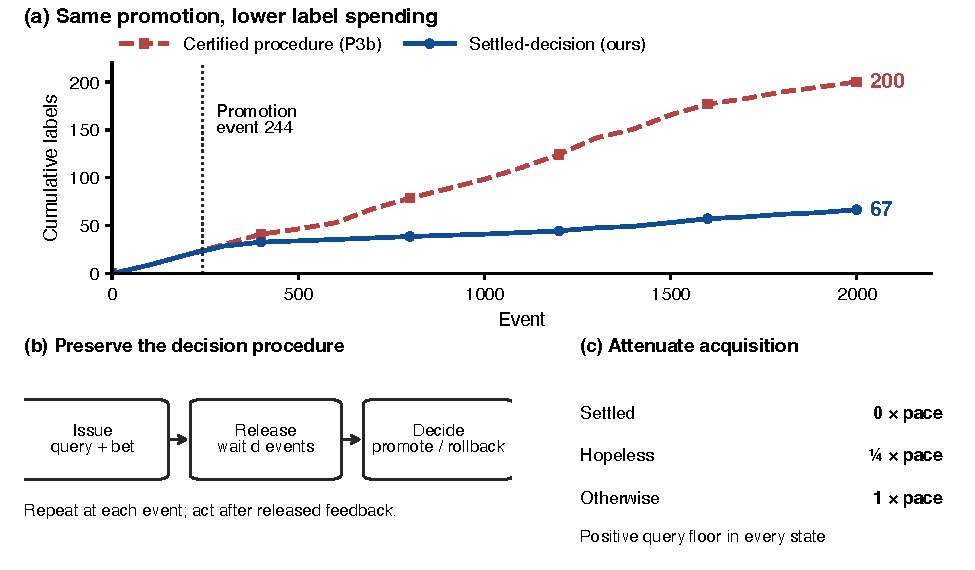
\includegraphics[width=\linewidth]{figures/fig1_method.pdf}
\caption{On the \texttt{spam} running example, settled-decision acquisition uses 67 labels per
episode in total instead of 200, with the same deployment summaries. (a) Cumulative requested
labels, sampled every 100 events (markers every 400) and averaged over 100 paired query seeds; the vertical line marks mean
promotion at event~244. (b) The issue--release--decide loop. (c) State-dependent acquisition
multipliers; the positive propensity floor applies in all states.}
\label{fig:method}
\end{figure}

\section{Method}\label{sec:method}
We first state the budgeted certified switching procedure \textsf{P3b}, then show where its budget
goes, introduce the gate, and show that the error bound is preserved.

\paragraph{Certified switching.} Let $a$ be the deployed model and $\Delta_s=\ell_a[s]-\ell_{1-a}[s]$
the paired advantage of the other model at event $s$. A released label contributes the
importance-weighted increment $x_s=Q_s\Delta_s/q_s$ to the wealth $W_t=\prod_{s}(1+\lambda_s x_s)$,
where the product runs over released events of the current segment. The bet is
$\lambda_s=\mathrm{clip}\bigl(\hat\mu_s/(\hat m_s+\hat\mu^2_s),\,0,\,q_s/2\bigr)$, where
$\hat\mu_s$ and $\hat m_s$ are discounted ($\gamma_b=0.99$) means of the released increments and
of their squares, shrunk towards $0$ and $1$ by ten pseudo-observations. Since $\hat m_s$ is a
second moment, adding $\hat\mu_s^2$ makes this a more conservative fraction than
aGRAPA~\citep{waudbysmith2024betting}; validity needs only a predictable
$\lambda_s\in[0,q_s/2]$. The cap $q_s/2$ matches the
event's own propensity, so every wealth factor is at least $1/2$. When $\log W_t\ge\log(1/\alpha)$
the procedure switches to the other model. A switch starts a new segment: the roles of the two models
swap, $W$ and the bet statistics reset, and only labels issued after the switch count. Rollback is
therefore the same test run against the newly deployed model. Queries follow a budget pacer,
\begin{equation}\label{eq:pace}
  q_t=\mathrm{clip}\!\left(r_t\cdot\frac{\mathrm{rem}_t}{\widehat{\text{rate}}_t\,(T-t+1)},\;
  p_{\min},\;1\right),\qquad
  \widehat{\text{rate}}_t=\frac{\sum_{s<t}D_s+5}{t-1+20},
\end{equation}
where $\mathrm{rem}_t$ is the unspent budget and $\widehat{\text{rate}}_t$ is the disagreement rate
estimated with a prior rate of $0.25$ worth 20 events. \textsf{P3b}, the ungated procedure, uses
$r_t\equiv1$.

\paragraph{Where the budget goes.} In the configuration of Section~\ref{sec:setup}, under
\textsf{P3b} mean promotion time is event $244$ on
\texttt{spam} (over 100 query seeds) and event $425$ on \texttt{rialto} (mean of its 16 episode
means; median $352$). On both streams every query seed of every episode promotes, after which querying continues at the
paced rate for most of the remaining horizon.

\paragraph{Settled-decision acquisition.} The gate changes only $r_t$. Let
$A_t$ be the recent discounted paired advantage, an exponential average ($\gamma_A=0.97$) of the
released increments of the current segment, so $A_t<0$ means the deployed model has recently been
ahead. While the incumbent is deployed, we run mirrored e-processes on a grid of margins
$m\in\{0,0.01,\dots,0.30\}$ for the nulls $\mathbb{E}[\Delta]\ge m$, started at ten staggered offsets 150 events apart and
tested at $\log(10/\alpha)$; the upper bound $\mathrm{UCB}_t$ is the smallest rejected margin, or
1 if none is rejected. Two states are gated:
\textsc{settled}, when the challenger is deployed and $A_t<0$; and \textsc{hopeless}, when the
incumbent is deployed, $A_t<0$ and $\mathrm{UCB}_t\,(T-t+1)<c_s$, so that even if the advantage
stayed at its upper bound for the rest of the horizon, promotion would not repay its switching
cost. With margins in steps of $0.01$ and $c_s=5$, this condition can hold more than 500 events
before the horizon only when the margin-0 null is rejected, that is, when the challenger has itself
been certified no better than the incumbent; \textsc{hopeless} therefore fires early only when
promotion is already implausible. The bound is a heuristic signal for acquisition; validity does
not depend on it. Then
\begin{equation}\label{eq:rule}
  r_t=\begin{cases}
    0 & \textsc{settled}\\
    0.25 & \textsc{hopeless}\\
    1 & \text{otherwise.}
  \end{cases}
\end{equation}
Since $r_t\le 1$, the gate only attenuates the paced query probability in each state. A settled
multiplier of $0$ still queries at $p_{\min}$ because $q_t$ is clipped there, so rollback
monitoring continues; when $A_t$ turns non-negative, a reversal signal, the full paced rate
returns. In \textsc{settled}, a disagreement rate $\rho$ gives $p_{\min}\rho$ labels per event in
expectation, so after a reversal the first label arrives after about $1/(p_{\min}\rho)$ events,
80 for $\rho=0.25$, and becomes usable $d$ events later. This expected waiting time is a lower
bound on the extra delay that reduced monitoring adds before the full rate can return, since one
label need not turn $A_t$ non-negative.

\begin{algorithm}[t]
\caption{Settled-decision acquisition (one event)}
\label{alg:main}
\begin{algorithmic}[1]
\STATE {\bfseries Issue:} compute $r_t$ by Eq.~\eqref{eq:rule} and $q_t$ by Eq.~\eqref{eq:pace}
from labels of events up to $t-d-1$; freeze $\lambda_t$ with the cap $q_t/2$.
\STATE Query iff $D_t=1$, $u_t<q_t$ and $\mathrm{rem}_t>0$.
\STATE {\bfseries Release:} if $s=t-d\ge1$ and $s$ lies in the current segment, multiply $W$ by
$1+\lambda_s x_s$ and update $A$ and the margin grids.
\STATE {\bfseries Decide:} if $\log W_t\ge\log(1/\alpha)$, switch the deployed model and start a
new segment, effective from $t+1$.
\end{algorithmic}
\end{algorithm}

\paragraph{Validity.} Acquisition changes which labels are bought, not how evidence is
accumulated. Let $\mathcal{G}_s$ be generated by the losses and query seeds of events up to $s$.

\begin{proposition}\label{prop:validity}
Fix a segment with deployed model $a$, started at a stopping time $\sigma$. Suppose that under the
null $H_0$, $\mathbb{E}[\Delta_s\mid\mathcal{G}_{s-1}]\le0$ for every event $s\ge\sigma$, and that
$u_s$ is independent of $\mathcal{G}_{s-1}$ and of the losses at $s$. If $q_s$, $\lambda_s$ and
$r_s$ are $\mathcal{G}_{s-1}$-measurable, $q_s>0$ whenever a label may be requested and
$0\le\lambda_s\le q_s/2$, then $\Pr_{H_0}\bigl(\exists t:\log W_t\ge\log(1/\alpha)\bigr)\le\alpha$.
In particular, the bound holds for every predictable choice of the acquisition multiplier $r_t$.
\end{proposition}

\begin{proof}
Given $\mathcal{G}_{s-1}$ and the losses at $s$, $\mathbb{E}[Q_s/q_s]=D_s\mathbf{1}\{\mathrm{rem}_s>0\}$,
and $\Delta_s=0$ when $D_s=0$, so $\mathbb{E}[x_s\mid\mathcal{G}_{s-1}]=\mathbf{1}\{\mathrm{rem}_s>0\}
\,\mathbb{E}[\Delta_s\mid\mathcal{G}_{s-1}]\le0$. Since $|x_s|\le1/q_s$ and $\lambda_s\le q_s/2$,
each factor $1+\lambda_s x_s$ lies in $[1/2,3/2]$, and $\lambda_s\ge0$ is predictable, so the
product over $s\ge\sigma$ is a non-negative supermartingale with initial value 1. Ville's
inequality bounds the probability that it ever reaches $1/\alpha$ by $\alpha$; the wealth observed
at event $t$ is this product up to $t-d$. The multiplier $r_s$ enters only through $q_s$, which is
predictable.
\end{proof}

In our replay the losses are fixed and only the query seeds are random, so $H_0$ reduces to
$\Delta_s\le0$ for every event of the segment; the replay therefore measures cost, while the
type-I guarantee concerns the stochastic-loss model of the proposition. The floor $p_{\min}$ is not needed for validity; it
keeps the test able to accumulate evidence and keeps rollback monitoring active.

\section{Experimental Setup}\label{sec:setup}
The experiments ask how many labels and how much net cost the gate saves relative to \textsf{P3b}
(Section~\ref{sec:results}), where the saving comes from (Sections~\ref{sec:results}
and~\ref{sec:ablation}), and how it depends on $c_q$, $c_s$, $B$ and $d$
(Section~\ref{sec:ablation}). The evaluation contains \NStreams{} real datasets, each giving one loss stream, and \NEpisodes{}
episodes: nine electricity meters from the UCI electricity load diagrams~\citep{trindade2015electricity},
five Beijing air-quality stations~\citep{zhang2017cautionary} and the Italian air-quality CO
series~\citep{devito2008field}, two demand and mobility series (\texttt{metro}~\citep{hogue2019metro}
and \texttt{bike\_hour}~\citep{fanaee2014event}), the \texttt{rialto} bridge time-lapse
stream~\citep{losing2016knn}, the \texttt{spam} email stream~\citep{katakis2010tracking} and the
localization-data-for-person-activity stream \texttt{openml\_ldpa} (OpenML
1483;~\citealp{kaluza2010agent}).

Continuous targets (meter load, pollutant concentration, traffic volume and bike counts) are
binarised at their median over the first 30\% of the series; \texttt{rialto} and
\texttt{openml\_ldpa} are reduced to their majority class against the rest, and \texttt{spam} is
spam against legitimate mail. Each stream uses a frozen incumbent--challenger pair fitted within the
first 30\% of the series: the incumbent on the first 15\% and the challenger on the first 30\%, with
label thresholds and preprocessing also fitted on the first 30\%. On the meter,
air-quality, demand and \texttt{rialto} streams the incumbent is logistic regression and the
challenger a gradient-boosted tree model; on \texttt{spam} both are logistic regressions; on
\texttt{openml\_ldpa} the challenger is a gradient-boosted tree model fitted on the first 30\%. Episodes are
2000-event windows taken after the first 30\%, at most 20 per stream for the meter, air-quality and
demand streams; $K$ denotes the
number of episodes of a stream, and \texttt{rialto}, \texttt{spam} and \texttt{openml\_ldpa}
contribute 16, 1 and 32.

The primary configuration is $T=2000$, $B=200$, $c_q=0.05$, $c_s=5$, $\alpha=0.05$ and
$p_{\min}=0.05$, with a fixed label delay per stream (24, 50, 96 or 100 events), and 100
query-randomisation seeds shared across policies. We compare settled-decision acquisition
(ours) with three policies on the same episodes and seeds: $P_0$, which never switches;
\textsf{P3b}, the ungated certified procedure of Section~\ref{sec:method}, which differs from ours
only in $r_t$; and \textsf{P6}, which queries disagreements with \textsf{P3b}'s pacing and runs a
single exact binomial (McNemar) test~\citep{mcnemar1947note} on the first 50 released disagreement
labels, promoting on rejection and never rolling back. The ablation also includes cost-aware
promotion (\textsf{P4ref}), which keeps \textsf{P3b}'s acquisition but promotes only when the
certificate fires and a single-offset lower confidence bound on the advantage, multiplied by a
declared persistence horizon of $\min(150,T-t)$ events, exceeds $c_s$.

\paragraph{Aggregation and uncertainty.}
Policy costs and label counts are averaged over query seeds, then over episodes within a stream.
The headline results are arithmetic means of the percentage reduction relative to \textsf{P3b},
computed separately for each dataset, with equal weight per dataset; medians of the same
reductions are reported alongside them. We report paired 95\% episode-bootstrap intervals, which
resample episodes rather than query seeds, using 10,000 resamples when a stream has at least five
episodes; this excludes \NLowPower{} streams. Two policies have matching deployment summaries on an episode when deployment loss,
switch count and rollback count agree on every query seed.

\section{Results}\label{sec:results}
\begin{figure}[!t]
\centering
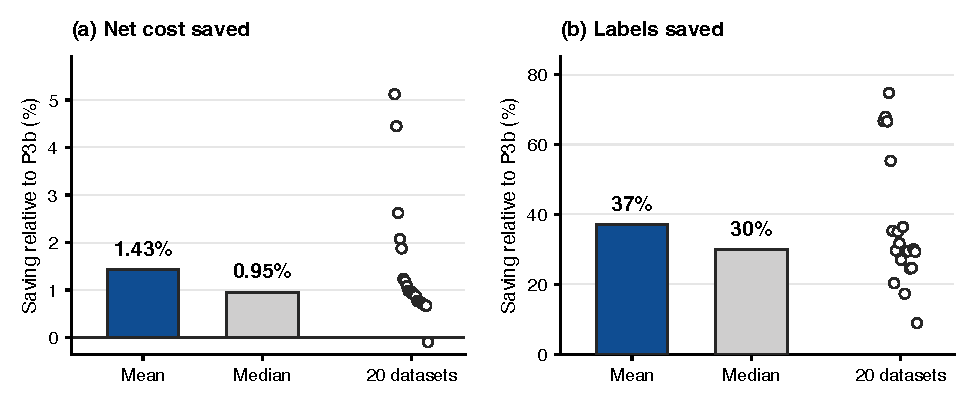
\includegraphics[width=\linewidth]{figures/fig4_all_streams.pdf}
\caption{Settled-decision acquisition saves \MeanSaving\% of labels and \MeanCostChange\% of net
cost on average across \NStreams{} datasets. Bars show the arithmetic mean and median of
dataset-level percentage reductions relative to \textsf{P3b} for net cost (a) and labels (b);
hollow points show all dataset values. The median savings are \MedSaving\% for labels and
\MedCostChange\% for net cost.}
\label{fig:all}
\end{figure}

Figure~\ref{fig:all} reports the headline result: averaged equally across \NStreams{} datasets,
settled-decision acquisition uses \MeanSaving\% fewer labels than \textsf{P3b} (median
\MedSaving\%, up to \MaxSaving\%), and deployment summaries match in \NSameEpisodes{} of
\NEpisodes{} episodes and in all episodes of \NSameStreams{} streams. Net cost is lower on
\NCheaper{} datasets and higher on \NDearer{}, by \MeanCostChange\% on average (median
\MedCostChange\%).

\begin{table}[!t]\centering\footnotesize\setlength{\tabcolsep}{4pt}
\caption{Primary results for every real dataset. Net cost and labels are means per episode.
Positive cost saved means ours is cheaper than \textsf{P3b}. Costs use unrounded records; label
counts are rounded only for display.}
\label{tab:main}
\begin{tabular}{lrrrrrrr}
\toprule
Stream & $K$ & $P_0$ & P3b & P6 & Ours & Cost saved & Labels P3b$\to$ours \\
\midrule
rialto & 16 & 202.06 & 103.73 & 122.91 & 98.42 & +5.12\% & 159$\to$53 \\
metro & 16 & 719.88 & 152.51 & 255.90 & 145.73 & +4.45\% & 200$\to$64 \\
spam & 1 & 849.00 & 254.09 & 315.95 & 247.43 & +2.62\% & 200$\to$67 \\
air\_quality\_co & 2 & 438.00 & 321.40 & 331.80 & 314.73 & +2.07\% & 178$\to$45 \\
bike\_hour & 6 & 552.83 & 292.16 & 331.52 & 286.68 & +1.88\% & 198$\to$89 \\
elec\_MT\_010 & 20 & 630.00 & 325.61 & 378.15 & 321.60 & +1.23\% & 162$\to$105 \\
air\_Tiantan & 12 & 335.00 & 310.50 & 306.39 & 306.82 & +1.19\% & 173$\to$138 \\
air\_Dingling & 12 & 275.50 & 266.02 & 265.82 & 263.13 & +1.09\% & 154$\to$108 \\
elec\_MT\_022 & 20 & 291.20 & 255.53 & 255.32 & 253.01 & +0.98\% & 144$\to$93 \\
air\_Dongsi & 12 & 342.33 & 324.27 & 334.21 & 321.11 & +0.98\% & 173$\to$118 \\
elec\_MT\_002 & 20 & 199.65 & 177.78 & 180.03 & 176.12 & +0.93\% & 122$\to$89 \\
openml\_ldpa & 32 & 663.00 & 483.25 & 506.51 & 478.82 & +0.92\% & 181$\to$115 \\
air\_Wanliu & 12 & 289.42 & 282.48 & 290.37 & 280.00 & +0.88\% & 187$\to$154 \\
air\_Shunyi & 11 & 359.27 & 345.35 & 338.31 & 342.70 & +0.77\% & 169$\to$119 \\
elec\_MT\_011 & 20 & 354.80 & 320.56 & 317.59 & 318.12 & +0.76\% & 161$\to$114 \\
elec\_MT\_014 & 20 & 284.85 & 255.11 & 255.28 & 253.24 & +0.73\% & 153$\to$115 \\
elec\_MT\_043 & 20 & 224.75 & 212.29 & 210.21 & 210.77 & +0.71\% & 123$\to$93 \\
elec\_MT\_027 & 20 & 370.65 & 352.15 & 346.45 & 349.76 & +0.68\% & 159$\to$111 \\
elec\_MT\_009 & 20 & 509.60 & 411.09 & 415.76 & 408.33 & +0.67\% & 185$\to$131 \\
elec\_MT\_041 & 15 & 212.20 & 228.61 & 229.82 & 228.83 & -0.09\% & 147$\to$134 \\
\bottomrule
\end{tabular}

\end{table}

Table~\ref{tab:main} reports every dataset, and Figures~\ref{fig:netcost} and~\ref{fig:labels}
show the dataset-level savings. The largest percentage savings are on \texttt{rialto} (5.12\%),
\texttt{metro} (4.45\%) and \texttt{spam} (2.62\%). The largest label saving is on
\texttt{air\_quality\_co}, from 178 to 45 labels per episode (75\%).

\begin{figure}[!t]
\centering
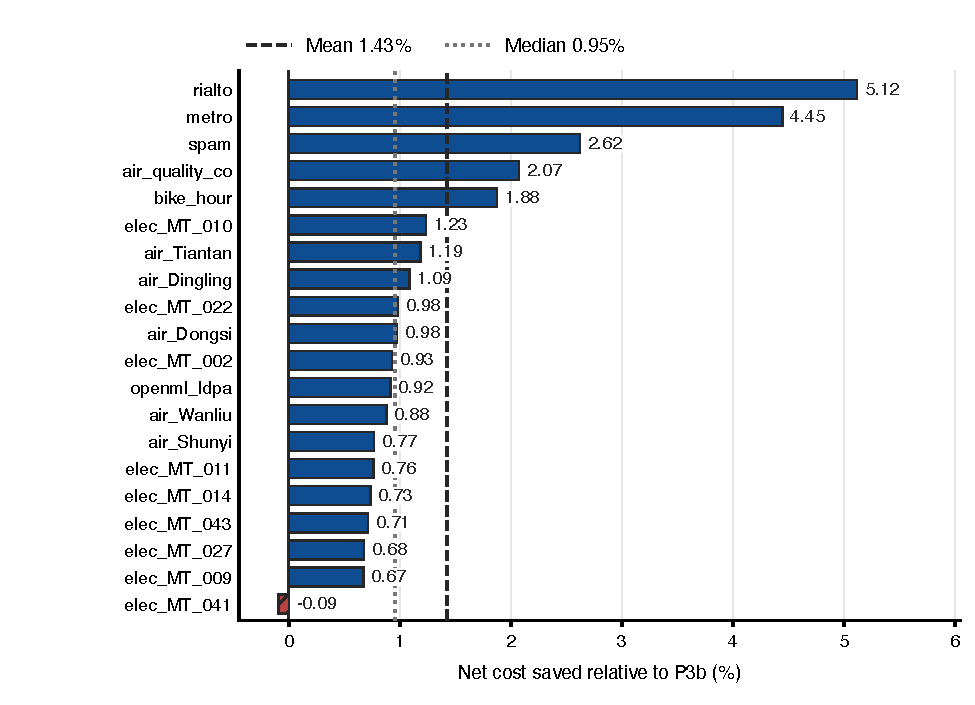
\includegraphics[width=\linewidth]{figures/fig2_netcost.pdf}
\caption{Net cost is \MeanCostChange\% lower on average across \NStreams{} datasets
(median \MedCostChange\%). Bars show each dataset's percentage reduction relative to \textsf{P3b};
negative values indicate increased cost. Dashed and dotted lines mark the mean and median,
respectively. Episode-bootstrap intervals for cost differences are in Appendix~\ref{app:streams}.}
\label{fig:netcost}
\end{figure}
\begin{figure}[!t]
\centering
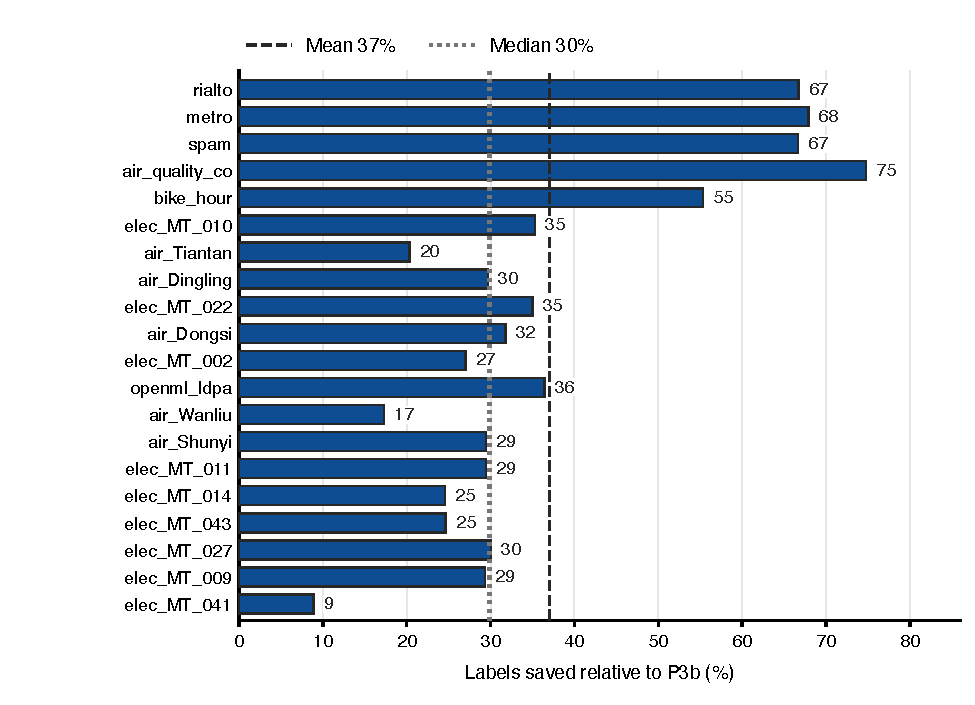
\includegraphics[width=\linewidth]{figures/fig3_labels.pdf}
\caption{Settled-decision acquisition uses \MeanSaving\% fewer labels on average
(median \MedSaving\%). Bars show the share of \textsf{P3b}'s labels saved on each of the
\NStreams{} datasets, in the order of Figure~\ref{fig:netcost}. Dashed and dotted lines mark the
mean and median, respectively.}
\label{fig:labels}
\end{figure}

\paragraph{Where the saving comes from.} Appendix~\ref{app:streams} decomposes each cost
difference. The gate never increases switching cost: the switch-cost difference is zero or
negative on every stream. On 10 streams the whole saving is query cost. On the other 10 the gate
buys less evidence and switches less often: switch cost falls on all 10, and deployment loss falls
on 7 (for example \texttt{air\_Tiantan}, $-1.36$ against a query difference of $-1.76$),
consistent with some of the ungated procedure's extra labels triggering switches that did not pay
off. On the remaining 3 (\texttt{air\_Dongsi}, \texttt{air\_Shunyi} and \texttt{elec\_MT\_041})
loss rises, consistent with either slower reversal detection under floor-rate monitoring
(Section~\ref{sec:method}) or \textsc{hopeless} delaying a promotion.
On \texttt{elec\_MT\_041} the loss increase ($+1.18$) outweighs the query ($-0.65$) and switch
($-0.31$) savings, so net cost rises by 0.09\%. Separately, never switching (212.20) is cheaper
than both certified procedures (228.61 and 228.83) on that stream, and more expensive than both on
the other 19.

\begin{table}[!htb]\centering\footnotesize\setlength{\tabcolsep}{2.5pt}
\caption{Results by source family. Cheaper/equal/dearer compares ours with \textsf{P3b}. Matching
summaries is the share of episodes with matching deployment summaries. P6 cheaper counts streams
where \textsf{P6} has lower mean cost than ours.}
\label{tab:families}
\begin{tabular}{lrrrrrr}
\toprule
Family & Streams & Episodes & Median labels saved & Cheaper / equal / dearer & Matching summaries & P6 cheaper \\
\midrule
Electricity meters & 9 & 175 & 29\% & 8 / 0 / 1 & 95\% & 3 \\
Air quality & 6 & 61 & 30\% & 6 / 0 / 0 & 75\% & 2 \\
Demand and mobility & 2 & 22 & 62\% & 2 / 0 / 0 & 100\% & 0 \\
Other real streams & 3 & 49 & 67\% & 3 / 0 / 0 & 84\% & 0 \\
\midrule
All & 20 & 307 & 30\% & 19 / 0 / 1 & 90\% & 5 \\
\bottomrule
\end{tabular}

\end{table}

Table~\ref{tab:families} breaks the result down by source family. \textsf{P6} is cheaper than ours
on \NSixCheaper{} streams. It differs from both certified procedures in its test and in its
monitoring: it runs one fixed-sample test on 50 labels and never rolls back. The comparison with
the certified procedures therefore concerns deployments that require rollback, which \textsf{P6}
does not provide.

\section{Mechanism and Ablations}\label{sec:ablation}
\begin{table}[!t]\centering\small
\caption{Ablation on \texttt{spam} and \texttt{rialto} under the primary configuration; $\Delta$ is
the paired cost difference against \textsf{P3b}.}
\label{tab:ablation}
\begin{tabular}{lrrrr}
\toprule
& \multicolumn{2}{c}{spam ($K=1$)} & \multicolumn{2}{c}{rialto ($K=16$)} \\
Variant & Cost & $\Delta$ & Cost & $\Delta$ \\
\midrule
Incumbent certified switching & 254.09 & $+0.00$ & 103.73 & $+0.00$ \\
Cost-aware promotion & 381.96 & $+127.87$ & 210.02 & $+106.29$ \\
Acquisition: \textsc{hopeless} only & 254.09 & $+0.00$ & 103.73 & $+0.00$ \\
Acquisition: both states & 247.43 & $-6.66$ & 98.42 & $-5.31$ \\
\bottomrule
\end{tabular}

\end{table}

This section isolates which state produces the saving, compares gating acquisition with gating
promotion, and varies $B$, $c_s$, $d$ and $c_q$. Both \texttt{spam} and \texttt{rialto} promote
early, so the \textsc{hopeless}-only variant leaves cost unchanged and the saving on these streams
is entirely due to the \textsc{settled} state (Table~\ref{tab:ablation}). Deployment loss,
switches and rollbacks match there, so the cost difference is entirely query cost. Cost-aware
promotion with a declared horizon of 150 events delays a promotion that pays off and costs
$+127.87$ and $+106.29$ on these streams, whereas gating acquisition leaves the decision intact.

\begin{table}[!htb]\centering\small
\caption{Sensitivity of the paired cost difference (ours minus \textsf{P3b}) on \texttt{spam},
\texttt{rialto} and \texttt{openml\_ldpa}. S0 is the primary configuration; dashes mark a
configuration not evaluated.}
\label{tab:sens}
\begin{tabular}{lrrrrr}
\toprule
Stream & S0 & S1 ($B=400$) & S2 ($c_s=20$) & S3 ($2\times d$) & S4 ($c_q=0.10$) \\
\midrule
spam & $-6.66$ & $-15.62$ & $-6.66$ & $-6.18$ & $-13.32$ \\
rialto & $-5.31$ & $-5.43$ & $-5.31$ & $-4.14$ & $-10.62$ \\
openml\_ldpa & $-4.43$ & $-11.48$ & $-5.29$ & \textemdash & $-7.73$ \\
\bottomrule
\end{tabular}

\end{table}

\paragraph{Sensitivity.}
Neither policy uses $c_q$, and only \textsc{hopeless} uses $c_s$. On \texttt{spam} and
\texttt{rialto} deployment is identical, and the unchanged S2 entries show that \textsc{hopeless}
does not change the outcome at $c_s=20$ either, although at $c_s=20$ a bound of $0.01$ would
satisfy its condition from the second event on. By Eq.~\eqref{eq:netcost} the difference there then
doubles exactly at $c_q=0.10$ (Table~\ref{tab:sens}). On \texttt{openml\_ldpa} the gate also lowers deployment loss
($-0.82$) and switch cost ($-0.30$, Appendix~\ref{app:streams}), and the $c_s=20$ and $c_q=0.10$
entries match that decomposition ($-0.82-3.30+4(-0.30)\approx-5.3$ and
$-0.82+2(-3.30)-0.30\approx-7.7$), so the saving there combines label spend with a deployment
change.

Since neither policy uses $c_q$, deployment does not depend on it, and each stream's cost difference at fixed $c_s$ and $B$
is $\Delta_{\text{loss}}+\Delta_{\text{switch}}+(c_q/0.05)\,\Delta_{\text{query}}$ in the terms of
Appendix~\ref{app:streams}. Only \texttt{elec\_MT\_041} has a positive
$\Delta_{\text{loss}}+\Delta_{\text{switch}}$ ($+0.87$) against a query saving of $0.65$, so it
breaks even at $c_q\approx0.067$. At $c_s=5$ and $B=200$ the gate is therefore cheaper than
\textsf{P3b} on all \NStreams{} datasets for any $c_q$ above that value.

Doubling the label delay changes the cost difference to $-6.18$ on \texttt{spam} and $-4.14$ on
\texttt{rialto}, consistent with a longer delay leaving fewer post-promotion events in which
\textsc{settled} withholds queries. The benefit depends on unspent budget that \textsf{P3b} would
otherwise consume: raising $B$ to $400$ increases the gain on \texttt{spam} and
\texttt{openml\_ldpa}, but leaves \texttt{rialto} essentially unchanged: its disagreement rate caps
queries near $165$, so the larger budget does not bind.

\section{Limitations}\label{sec:limits}
Streams within a family are correlated, so stream counts are descriptive rather than independent
trials. Episodes of one stream are windows of the same series and may be temporally dependent, so
the episode bootstrap may understate uncertainty; of the streams, \NLowPower{} contribute fewer
than five episodes and have no interval. The gate's settings ($\gamma_A$, the \textsc{hopeless} multiplier, the margin
grid and $p_{\min}$) are not varied. Reduced post-promotion monitoring rests on the floor-rate queries and
can detect a reversal later than \textsf{P3b}. The contribution of the \textsc{hopeless} state is
not isolated: the ablation streams promote early, and on the remaining streams its effect is not
separated from that of the \textsc{settled} state. Proposition~\ref{prop:validity} controls the error of each certificate segment; it
does not bound errors accumulated over a sequence of promotions and rollbacks, each of which
restarts at the threshold $\log(1/\alpha)$. Matching deployment summaries do not imply identical
event-by-event actions. The event order of \texttt{openml\_ldpa} is inferred from undocumented
columns, and its non-stationarity largely reflects changes of recorded subject between blocks.

\section{Conclusion}
On \texttt{spam} the ungated procedure spent its full 200-label budget, most of it after
promotion at event 244; settled-decision acquisition spent 67 with the same deployment
summaries. Across \NStreams{} real datasets the
gate uses \MeanSaving\% fewer labels (median \MedSaving\%) and lowers net cost on \NCheaper{} of
them, by \MeanCostChange\% on average (median \MedCostChange\%), while the certificate and its type-I
error guarantee are retained and rollback monitoring continues at the floor rate $p_{\min}$. The
saving grows with the label price: in this configuration the gate is cheaper on every dataset once
a label costs more than about $0.067$.

\bibliography{references}
\bibliographystyle{tmlr}

\clearpage
\appendix
\section{Per-Stream Cost Decomposition}\label{app:streams}
{\footnotesize\setlength{\tabcolsep}{3pt}\begin{longtable}{lrrrrrr}
\caption{Per-stream differences (ours minus P3b). Intervals use 10,000 paired episode-bootstrap resamples; dashes indicate fewer than five episodes.}\label{tab:streams}\\
\toprule
Stream & $d$ & $\Delta$ cost & 95\% episode interval & $\Delta$ loss & $\Delta$ query cost & $\Delta$ switch cost \\
\midrule
\endfirsthead
\toprule
Stream & $d$ & $\Delta$ cost & 95\% episode interval & $\Delta$ loss & $\Delta$ query cost & $\Delta$ switch cost \\
\midrule
\endhead
\bottomrule
\endlastfoot
rialto & 100 & $-5.31$ & $[-5.98,-4.61]$ & $+0.00$ & $-5.31$ & $+0.00$ \\
metro & 24 & $-6.78$ & $[-6.95,-6.60]$ & $+0.00$ & $-6.78$ & $+0.00$ \\
spam & 50 & $-6.66$ & \textemdash & $+0.00$ & $-6.66$ & $+0.00$ \\
air\_quality\_co & 24 & $-6.67$ & \textemdash & $+0.00$ & $-6.67$ & $+0.00$ \\
bike\_hour & 24 & $-5.48$ & $[-6.46,-4.28]$ & $+0.00$ & $-5.48$ & $+0.00$ \\
elec\_MT\_010 & 96 & $-4.02$ & $[-6.82,-2.17]$ & $-0.97$ & $-2.86$ & $-0.19$ \\
air\_Tiantan & 24 & $-3.68$ & $[-6.54,-1.27]$ & $-1.36$ & $-1.76$ & $-0.56$ \\
air\_Dingling & 24 & $-2.89$ & $[-5.03,-1.06]$ & $-0.37$ & $-2.28$ & $-0.24$ \\
elec\_MT\_022 & 96 & $-2.51$ & $[-3.46,-1.57]$ & $+0.00$ & $-2.51$ & $+0.00$ \\
air\_Dongsi & 24 & $-3.16$ & $[-4.37,-1.98]$ & $+0.26$ & $-2.76$ & $-0.67$ \\
elec\_MT\_002 & 96 & $-1.65$ & $[-2.60,-0.79]$ & $+0.00$ & $-1.65$ & $+0.00$ \\
openml\_ldpa & 100 & $-4.43$ & $[-7.04,-2.64]$ & $-0.82$ & $-3.30$ & $-0.30$ \\
air\_Wanliu & 24 & $-2.48$ & $[-5.03,-0.70]$ & $-0.51$ & $-1.62$ & $-0.35$ \\
air\_Shunyi & 24 & $-2.66$ & $[-3.96,-1.39]$ & $+0.15$ & $-2.49$ & $-0.31$ \\
elec\_MT\_011 & 96 & $-2.45$ & $[-3.35,-1.51]$ & $-0.06$ & $-2.38$ & $-0.01$ \\
elec\_MT\_014 & 96 & $-1.87$ & $[-2.77,-1.03]$ & $+0.00$ & $-1.87$ & $+0.00$ \\
elec\_MT\_043 & 96 & $-1.51$ & $[-2.34,-0.74]$ & $+0.00$ & $-1.51$ & $+0.00$ \\
elec\_MT\_027 & 96 & $-2.39$ & $[-3.35,-1.46]$ & $+0.00$ & $-2.39$ & $+0.00$ \\
elec\_MT\_009 & 96 & $-2.77$ & $[-3.60,-1.86]$ & $-0.01$ & $-2.71$ & $-0.05$ \\
elec\_MT\_041 & 96 & $+0.22$ & $[-1.06,+2.31]$ & $+1.18$ & $-0.65$ & $-0.31$ \\
\end{longtable}
}
\end{document}
